%=====================================================================
%  IEEE journal manuscript. Compile with pdfLaTeX + BibTeX
%  Order:  pdfLaTeX -> BibTeX -> pdfLaTeX -> pdfLaTeX
%  Multimodal polysomnography: joint staging + respiratory-event detection.
%  Supervision draft: full benchmark, math formulation, expanded review.
%=====================================================================
\documentclass[journal]{IEEEtran}
% Avoid "TeX capacity exceeded [PDF object stream buffer]" that Overleaf/TeXLive raises
% on large embedded figures. Disabling object-stream compression sidesteps the buffer.
\ifdefined\pdfobjcompresslevel\pdfobjcompresslevel=0\fi
\IEEEoverridecommandlockouts
\usepackage{cite}
\usepackage{amsmath,amssymb,amsfonts}
\usepackage{algorithmic}
\usepackage{graphicx}
% resolve figures/ locally (../figures) and on Overleaf (./figures)
\graphicspath{{../}{./}}
\usepackage{textcomp}
\usepackage{xcolor}
\usepackage{booktabs}
\usepackage{array}
\usepackage{multirow}
\usepackage{url}
\usepackage{stfloats}   % lets two-column (starred) floats sit at the bottom of a page
% allow more (and wider) floats per page so the many two-column tables place near
% their references instead of piling up after the bibliography.
\setcounter{topnumber}{3}
\setcounter{totalnumber}{5}
\setcounter{dbltopnumber}{3}
\renewcommand{\topfraction}{0.95}
\renewcommand{\bottomfraction}{0.7}
\renewcommand{\dbltopfraction}{0.95}
\renewcommand{\textfraction}{0.05}
\renewcommand{\floatpagefraction}{0.7}
\renewcommand{\dblfloatpagefraction}{0.7}
\def\BibTeX{{\rm B\kern-.05em{\sc i\kern-.025em b}\kern-.08em T\kern-.1667em\lower.7ex\hbox{E}\kern-.125emX}}
\usepackage[colorlinks=true,citecolor=blue,linkcolor=blue,urlcolor=blue,breaklinks=true]{hyperref}

% Headline numbers -- live-reproduced by revision/MM_Net_reproduction.ipynb (10-fold).
\newcommand{\mmAcc}{0.722}
\newcommand{\mmMf}{0.651}
\newcommand{\mmK}{0.611}
\newcommand{\mmAuc}{0.711}
\newcommand{\mmAp}{0.337}
\newcommand{\eegAuc}{0.673}
\newcommand{\noflowAuc}{0.704}

\begin{document}

\title{A Physiologically Interpretable Multimodal Model for Joint Sleep Staging and Respiratory-Event Detection in Subacute Ischemic Stroke}

\author{Md Wahiduzzaman Suva, Esm-e Moula Chowdhury Abha, Md Imtiaj Alam Sajin,
and Md Iftekharul Mobin%
\thanks{The authors are with the Department of Computer Science and Engineering,
American International University-Bangladesh, Dhaka, Bangladesh
(e-mail: 26-94088-2@student.aiub.edu; 26-94089-2@student.aiub.edu;
26-94090-2@student.aiub.edu; iftekhar.mobin@aiub.edu).}%
\thanks{Corresponding author: Md Iftekharul Mobin (iftekhar.mobin@aiub.edu).}}

\markboth{Manuscript, July 2026}%
{Suva \MakeLowercase{\textit{et al.}}: Multimodal Polysomnography in Ischemic Stroke}

\maketitle

%=====================================================================
% CONTRIBUTIONS -- placed before the abstract per submission requirement
\noindent\fcolorbox{black}{gray!8}{%
\parbox{0.955\columnwidth}{\footnotesize
\textbf{CONTRIBUTIONS.}\;
\textbf{Md Wahiduzzaman Suva} (Conceptualization, Methodology, Software,
Investigation, Validation, Formal analysis, Writing -- original draft, Project
administration): conceived the joint formulation and led the study; designed and
implemented MM-Net, the raw multimodal CNN and the ten-fold reproduction engine;
ran the joint staging--respiratory experiments, the modality-ablation grid and the
significance tests; led the verification pass; produced Tables~III--VI and wrote
Sections~I, V--VIII.\;
\textbf{Esm-e Moula Chowdhury Abha} (Investigation, Software, Validation,
Visualization, Writing -- original draft): trained and evaluated the deep
comparison models -- DeepSleepNet, AttnSleep and the healthy-pretrained transfer
model -- on matched folds; produced the architecture diagram (Fig.~3) via the
draw.io vector pipeline; wrote Sections~II--III; produced Table~VIII and compiled
the bibliography.\;
\textbf{Md Imtiaj Alam Sajin} (Data curation, Software, Investigation,
Visualization): built the polysomnography preprocessing pipeline -- channel
mapping, resampling, epoching -- and the feature extractors; trained the
respiratory reference detectors; produced Figures~4--10 and Tables~I, II
and~VII; wrote Section~IV.\;
\textbf{Md Iftekharul Mobin} (Supervision, Project administration,
Conceptualization, Writing -- review \& editing, Resources): supervised the
project and its clinical framing, critically revised the manuscript, and
provided institutional resources; corresponding author.
}}
\vspace{4pt}



%=====================================================================
\begin{abstract}
A clinical polysomnogram records far more than the brain. Alongside the
electroencephalogram it captures eye movements, muscle tone, the electrocardiogram,
nasal and oral airflow, thoracic and abdominal breathing effort, and blood oxygen
saturation. In patients recovering from ischemic stroke, a group in which breathing is
disturbed during sleep at high rates, these cardiorespiratory signals carry the disease
itself. We build one model that reads the full polysomnogram and produces two clinical
outputs at once: the sleep stage of every 30-second epoch and a per-epoch label for
respiratory events. The model encodes the neural and the cardiorespiratory signals in two
parallel streams, fuses them, follows the night with a bidirectional recurrent decoder, and
drives a staging head and a respiratory head, with a direct connection that carries the
cardiorespiratory signal to the respiratory head so oxygen desaturation reaches the decision at
full strength. We benchmark
the model against deep-learning and classical baselines on iSLEEPS, the first public
polysomnography corpus of subacute ischemic stroke (99 patients), all under patient-independent ten-fold
cross-validation. The single model stages sleep at $\mmAcc$ accuracy with Cohen's $\kappa$
of $\mmK$, at the accuracy ceiling this cohort imposes on every model family, and it detects
respiratory events at $\mmAuc$ area under the ROC curve, a capability none of the staging
models possess. The respiratory read-out is grounded in physiology: when we remove the
airflow channel from which the events were scored, detection holds at $\noflowAuc$, because
the model reads oxygen desaturation, breathing effort, cardiac variability, and the cortical
arousals that follow an obstructed breath. Each modality contributes where its physiology
lives. Code and features are released.
\end{abstract}

\begin{IEEEkeywords}
Polysomnography, multimodal learning, sleep staging, sleep apnea, ischemic stroke,
feature fusion, multi-task learning, cardiorespiratory signals.
\end{IEEEkeywords}

%=====================================================================
\section{Introduction}
\IEEEPARstart{S}{leep} is scored in 30-second epochs into five stages, Wake (W), N1, N2,
N3, and rapid-eye-movement (REM), following the American Academy of Sleep Medicine (AASM)
rules~\cite{aasm2023manual}. The overwhelming majority of automated methods read a single
electroencephalogram (EEG) channel and ask one question: how accurately can the five stages
be classified? Two decades of work on that question have moved from convolutional and
recurrent encoders~\cite{supratak2017deepsleepnet,phan2019seqsleepnet,supratak2020tinysleepnet}
through attention and sequence models~\cite{eldele2021attnsleep,phan2021xsleepnet,
perslev2019utime} to large self-supervised EEG foundation
models~\cite{labram2024,cbramod2025,eegpt2024,biot2023}. On healthy sleepers these methods
reach roughly $85\%$ accuracy, and recent reviews argue the field is near a ceiling set by
inter-scorer disagreement~\cite{phan2022survey}.

A clinical polysomnogram (PSG), however, is a recording of the whole sleeping body. It
carries the EEG, eye movements, muscle tone, the electrocardiogram (ECG), nasal and oral
airflow, thoracic and abdominal breathing effort, and peripheral oxygen saturation
(SpO$_2$). These cardiorespiratory channels are where sleep-disordered breathing writes
itself: a paused breath, a chest that keeps straining against a closed airway, a fall in
blood oxygen, and the arousal that rescues the breath. A model that reads only the EEG
cannot see any of this, and so cannot report on the disorder that most damages a patient's
sleep. We use the full polysomnogram, and we ask a question that the staging race does not:
what does a model gain, and on which clinical task, when it reads the whole recording rather
than the brain alone.

We study this on iSLEEPS~\cite{maiti2026isleeps}, released in 2026 as the first public PSG
corpus dedicated to subacute ischemic stroke. The cohort is well matched to the question.
Sleep-disordered breathing is common in the weeks after a stroke and is tied to worse
recovery~\cite{bassetti2006sleep,denis2024sleep}, and in this corpus the median patient
carries a scored respiratory event in $13\%$ of epochs, with $77$ of $96$ patients above
$5\%$ (Fig.~\ref{fig:prev}). The cardiorespiratory signal is therefore abundant and
clinically meaningful in exactly the population where breathing matters most. The published
staging baselines on this corpus reach $74.7\%$ accuracy for an LSTM, about ten points below
the healthy state of the art, and a concurrent study reports that deep networks attend to
non-physiological regions on this cohort~\cite{bose2026gap}, so the setting also stresses
every staging architecture we can bring to it.

We present a two-stream, multi-task model that treats staging and respiratory-event
detection as one joint problem, and we place it inside a broad benchmark on the same folds. Our
contributions are:

\begin{itemize}
\item[\textbf{C1.}] \textbf{One model for two clinical read-outs from the full polysomnogram.} It stages
sleep at $\mmAcc$ accuracy ($\kappa$ $\mmK$) and, from the same forward pass, detects
respiratory events at $\mmAuc$ AUC, with a direct cardiorespiratory path to the respiratory
head so oxygen-desaturation cues reach the decision undiminished (Section~\ref{sec:method}).
\item[\textbf{C2.}] \textbf{Healthy-sleep deep models fail on the injured brain.} Deep networks trained from
scratch, transferred from healthy sleep, or applied to the raw multichannel signal collapse to
$0.61$--$0.69$ accuracy on this cohort (Table~\ref{tab:bench}), while classical pipelines
saturate below $0.75$; the compact feature-based model reaches $\mmAcc$ and, uniquely, also
produces a respiratory read-out. Staging accuracy here reflects a cohort ceiling; the joint respiratory output is what we contribute.
\item[\textbf{C3.}] \textbf{A physiologically grounded respiratory read-out.}
Removing the airflow channel from which the events were scored leaves detection at
$\noflowAuc$ AUC, because the decision rests on oxygen desaturation, breathing effort,
cardiac variability, and cortical arousals (Section~\ref{sec:noflow}).
\item[\textbf{C4.}] \textbf{Causal, per-modality attribution.} A
leave-one-out modality-ablation grid shows each channel carries the task its physiology governs:
removing the cardiorespiratory stream lowers only respiratory detection (Wilcoxon $p=0.004$),
while removing the ocular channel lowers only staging, giving a falsifiable and physiologically
interpretable account of the model (Table~\ref{tab:ablate}).
\end{itemize}

Together, these results reframe the problem on this cohort: the useful gains come from reading
the whole sleeping body and attributing each output to the physiology that produces it;
deeper single-channel staging does not help on this cohort. The remainder of the paper develops the model
(Section~\ref{sec:method}) and tests each claim in turn.

%=====================================================================
\section{Related Work}
\label{sec:related}

\subsection{Single-channel deep sleep staging}
Automated staging matured on one EEG channel. DeepSleepNet paired convolutional feature
extraction with a bidirectional LSTM~\cite{supratak2017deepsleepnet}; SeqSleepNet framed the
night as sequence-to-sequence labeling~\cite{phan2019seqsleepnet}; AttnSleep introduced
attention over multi-resolution convolutions~\cite{eldele2021attnsleep}; TinySleepNet and
U-Time reduced the parameter budget while holding
accuracy~\cite{supratak2020tinysleepnet,perslev2019utime}; and XSleepNet fused raw and
spectral views~\cite{phan2021xsleepnet}. More recent backbones push this further: SleepTransformer
adds interpretability and uncertainty to an attention model~\cite{sleeptransformer2022}, L-SeqSleepNet
models whole-night cycles~\cite{lseqsleepnet2023}, ZleepAnlystNet and FlexSleepTransformer explore
separated training and flexible channel sets~\cite{jirakittayakorn2024zleep,guo2024flexsleep}, and
linear-time state-space backbones reach competitive accuracy~\cite{gu2023mamba,bitmamsleep2024}.
These models set the accuracy on healthy corpora but
depend on the cortical micro-events that stroke disturbs, which is why they transfer poorly to
patients~\cite{bose2026gap}.

\subsection{Multi-channel and foundation models}
Later work reads several PSG channels. U-Sleep stages from arbitrary EEG and EOG derivations
across many cohorts~\cite{perslev2021usleep}, and self-supervised EEG foundation models such
as LaBraM, CBraMod, EEGPT, and BIOT learn transferable representations from large unlabeled
corpora~\cite{labram2024,cbramod2025,eegpt2024,biot2023}. SleepFM extends this idea to several
PSG modalities~\cite{sleepfm2026}, while cross-scale foundation models and standardized
benchmarks continue to appear~\cite{csbrain2025,neuroatlas2026,sleepyland2026}, self-supervised
pretraining is now systematically evaluated for label efficiency~\cite{estevan2025ssl}, transfer
and domain adaptation improve robustness across cohorts~\cite{guillot2023transfer}, and recent
surveys and clinical benchmarks catalogue the field~\cite{yang2026review,hanif2025insomnia}. The eye and muscle channels help most with REM and Wake,
which a single EEG channel resolves poorly. Reported gains from adding respiratory channels to
\emph{staging} are small and cohort-dependent; our benchmark quantifies this directly on a
high-burden clinical cohort and separates the staging effect from the respiratory one.

\subsection{Detection of sleep-disordered breathing}
A parallel line of work detects apnea and hypopnea from breathing signals. Airflow and effort
shape, oximetry, and ECG-derived heart-rate variability are all informative, and oxygen
desaturation is a defining marker of an event~\cite{jing2025cpap}. These detectors usually run
at fine time resolution on the raw breathing waveforms and are trained on that task alone. We
instead detect respiratory events on the staging epoch grid, jointly with staging, from a
shared representation, so that one model produces both clinical outputs and the two tasks
support each other during training.

\subsection{Sleep and breathing after stroke}
Sleep is both disturbed by stroke and predictive of recovery, and sleep-disordered breathing
is common in the subacute phase and linked to poorer functional
outcome~\cite{bassetti2006sleep,denis2024sleep,tellenbach2023brainstem}. Focal injury also changes
the micro-events that scoring relies on, the spindles, slow waves, and muscle
atonia~\cite{gottselig2002stroke,fernandez2019spindles,simpson2023laterality,facchin2020slowwaves,zheng2025spindles};
quantitative EEG markers such as the brain symmetry index further track hemispheric
injury~\cite{anastasi2017bsi}. A model that reports on breathing as well as stage is therefore of
direct clinical value in this population. Sleep staging on ischemic stroke itself is nascent, reported only as baselines on
the iSLEEPS corpus~\cite{maiti2026isleeps}, and no prior method addresses staging and respiratory
detection jointly, from the full polysomnogram, on a stroke population; we make this comparison
quantitative in Table~\ref{tab:litreview}.

%=====================================================================
\section{Critical Gaps and Limitations of Prior Work}
\label{sec:gaps}
Three gaps run through the literature above, and each maps onto one of our contributions.
\emph{(i) Single-task, single-signal design.} Almost every staging model reads one or a few EEG
channels and predicts only the stage, while apnea detectors read breathing signals and predict
only events; the two literatures rarely meet in one model, leaving the clinician with two
separate tools. Contribution~C1 answers this with a single model that reads the full
polysomnogram and produces both outputs.
\emph{(ii) Evaluation on healthy sleepers.} Staging accuracy is reported almost entirely on
healthy corpora such as Sleep-EDF~\cite{kemp2000sleepedf,goldberger2000physionet}, where deep
and foundation models reach a ceiling, while performance on focal brain injury is largely
unmeasured. Contribution~C2 benchmarks strong deep architectures, classical gradient-boosting
pipelines~\cite{chen2016xgboost,ke2017lightgbm,prokhorenkova2018catboost}, and graph
models~\cite{velickovic2018gat} on a subacute-stroke cohort, and shows that the healthy-built
networks collapse.
\emph{(iii) Attribution, reliability, and cost.} Interpretability is usually post-hoc and
unfalsifiable, predictive uncertainty is seldom modeled~\cite{angelopoulos2023conformal}, and the
compute and energy footprint of heavy models is rarely reported~\cite{lacoste2019carbon}.
Contributions~C3 and~C4 answer this with a physiologically grounded, non-circular respiratory
read-out and a causal modality-ablation that attributes each output to the channel its physiology
governs, in a compact model.

%=====================================================================
\section{Dataset and Preprocessing}
\label{sec:data}
iSLEEPS~\cite{maiti2026isleeps} contains overnight PSG from 100 subacute ischemic-stroke
patients (mean age $50.5$; 77 male, 23 female), scored by experts into the five AASM stages.
We exclude one recording after an audit: the data records of SN28 are byte-identical to those
of SN15, a duplication consistent with the anonymization and re-numbering the dataset authors
describe, and keeping it would place a training subject into the test fold in nine of ten fold
assignments, giving $N=99$. Sleep staging uses all $99$ patients; the respiratory task uses
the $N=96$ with complete cardiorespiratory channels, and we state which $N$ applies to each
reported number. The corpus totals $89{,}532$ epochs. The stage distribution
(Table~\ref{tab:dist}) is strongly imbalanced, with N2 dominant and N1 and N3 scarce, which is
the clinical norm.

\begin{table}[t]
\caption{Stage distribution and respiratory-event prevalence in the corpus we model ($N=99$).}
\label{tab:dist}
\centering
\begin{tabular}{lccccc}
\toprule
Stage & W & N1 & N2 & N3 & R \\
\midrule
Share (\%) & 26.6 & 10.2 & 42.3 & 8.9 & 12.1 \\
\bottomrule
\end{tabular}
\\[2pt]
\footnotesize Respiratory events: $16.0\%$ of epochs positive; median $13\%$ per patient
(range $0$ to $60.5\%$); $77$ of $96$ patients above $5\%$.
\end{table}

\begin{figure}[t]
\centering
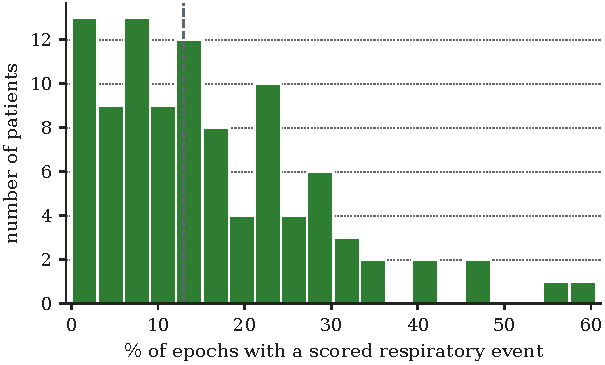
\includegraphics[width=0.86\columnwidth]{figures/fig_mm_apnea_prev.pdf}
\caption{Sleep-disordered-breathing burden across the cohort. Each bar counts patients by the
fraction of epochs that carry a scored respiratory event. The median patient sits at $13\%$
and many exceed $30\%$, so the cardiorespiratory signal is abundant.}
\label{fig:prev}
\end{figure}

\paragraph{Channels we read, and channels we do not}
A raw recording holds 22 traces. We read the 14 that carry sleep-stage or breathing
information. The \emph{neural stream} takes the four EEG derivations (C4:M1, C3:M2, O2:M1,
O1:M2), the two EOG channels (E1:M2, E2:M2), and the submental EMG. The
\emph{cardiorespiratory stream} takes the ECG, nasal and oral airflow, thoracic effort,
abdominal effort, the summed effort trace, SpO$_2$, and pulse. We leave out eight traces for
stated reasons: periodic limb movement records a different disorder; snore is scored from the
same airway sound as the respiratory events and would make the second task circular;
plethysmography is already summarized by the SpO$_2$ and pulse channels we keep; body position
is coarse and slow; and the ambient-light and battery traces are device housekeeping, not
physiology. All neural channels are resampled to $100$\,Hz and the cardiorespiratory channels
to a common $25$\,Hz grid; SpO$_2$, recorded natively at $4$\,Hz, is upsampled to this grid, so
its effective resolution remains that of the $4$\,Hz oximeter. Signals are read in physical
units, which matters because SpO$_2$ near $90\%$,
pulse near $78$\,bpm, and microvolt EEG live on very different scales. Per-epoch respiratory
labels are the corpus's scored events mapped onto the $30$\,s grid, and an epoch is positive
when it overlaps an event.

%=====================================================================
\section{Proposed Method}
\label{sec:method}
\subsection{Problem formulation}
A night is a sequence of $T$ epochs. For epoch $t$ we form a neural feature vector
$\mathbf{f}^{\mathrm{eeg}}_t\in\mathbb{R}^{188}$ and a cardiorespiratory feature vector
$\mathbf{f}^{\mathrm{car}}_t\in\mathbb{R}^{14}$, and we learn a subject-independent map
\begin{equation}
f_\theta:\big(\mathbf{f}^{\mathrm{eeg}}_{1:T},\mathbf{f}^{\mathrm{car}}_{1:T}\big)\ \longmapsto\
\big(\hat y^{\mathrm{stg}}_{1:T},\ \hat y^{\mathrm{apn}}_{1:T}\big),
\end{equation}
where $\hat y^{\mathrm{stg}}_t\in\Delta^4$ is a distribution over the five stages and
$\hat y^{\mathrm{apn}}_t\in[0,1]$ is the probability that epoch $t$ contains a respiratory
event (Fig.~\ref{fig:arch}).

\begin{figure*}[t]
\centering
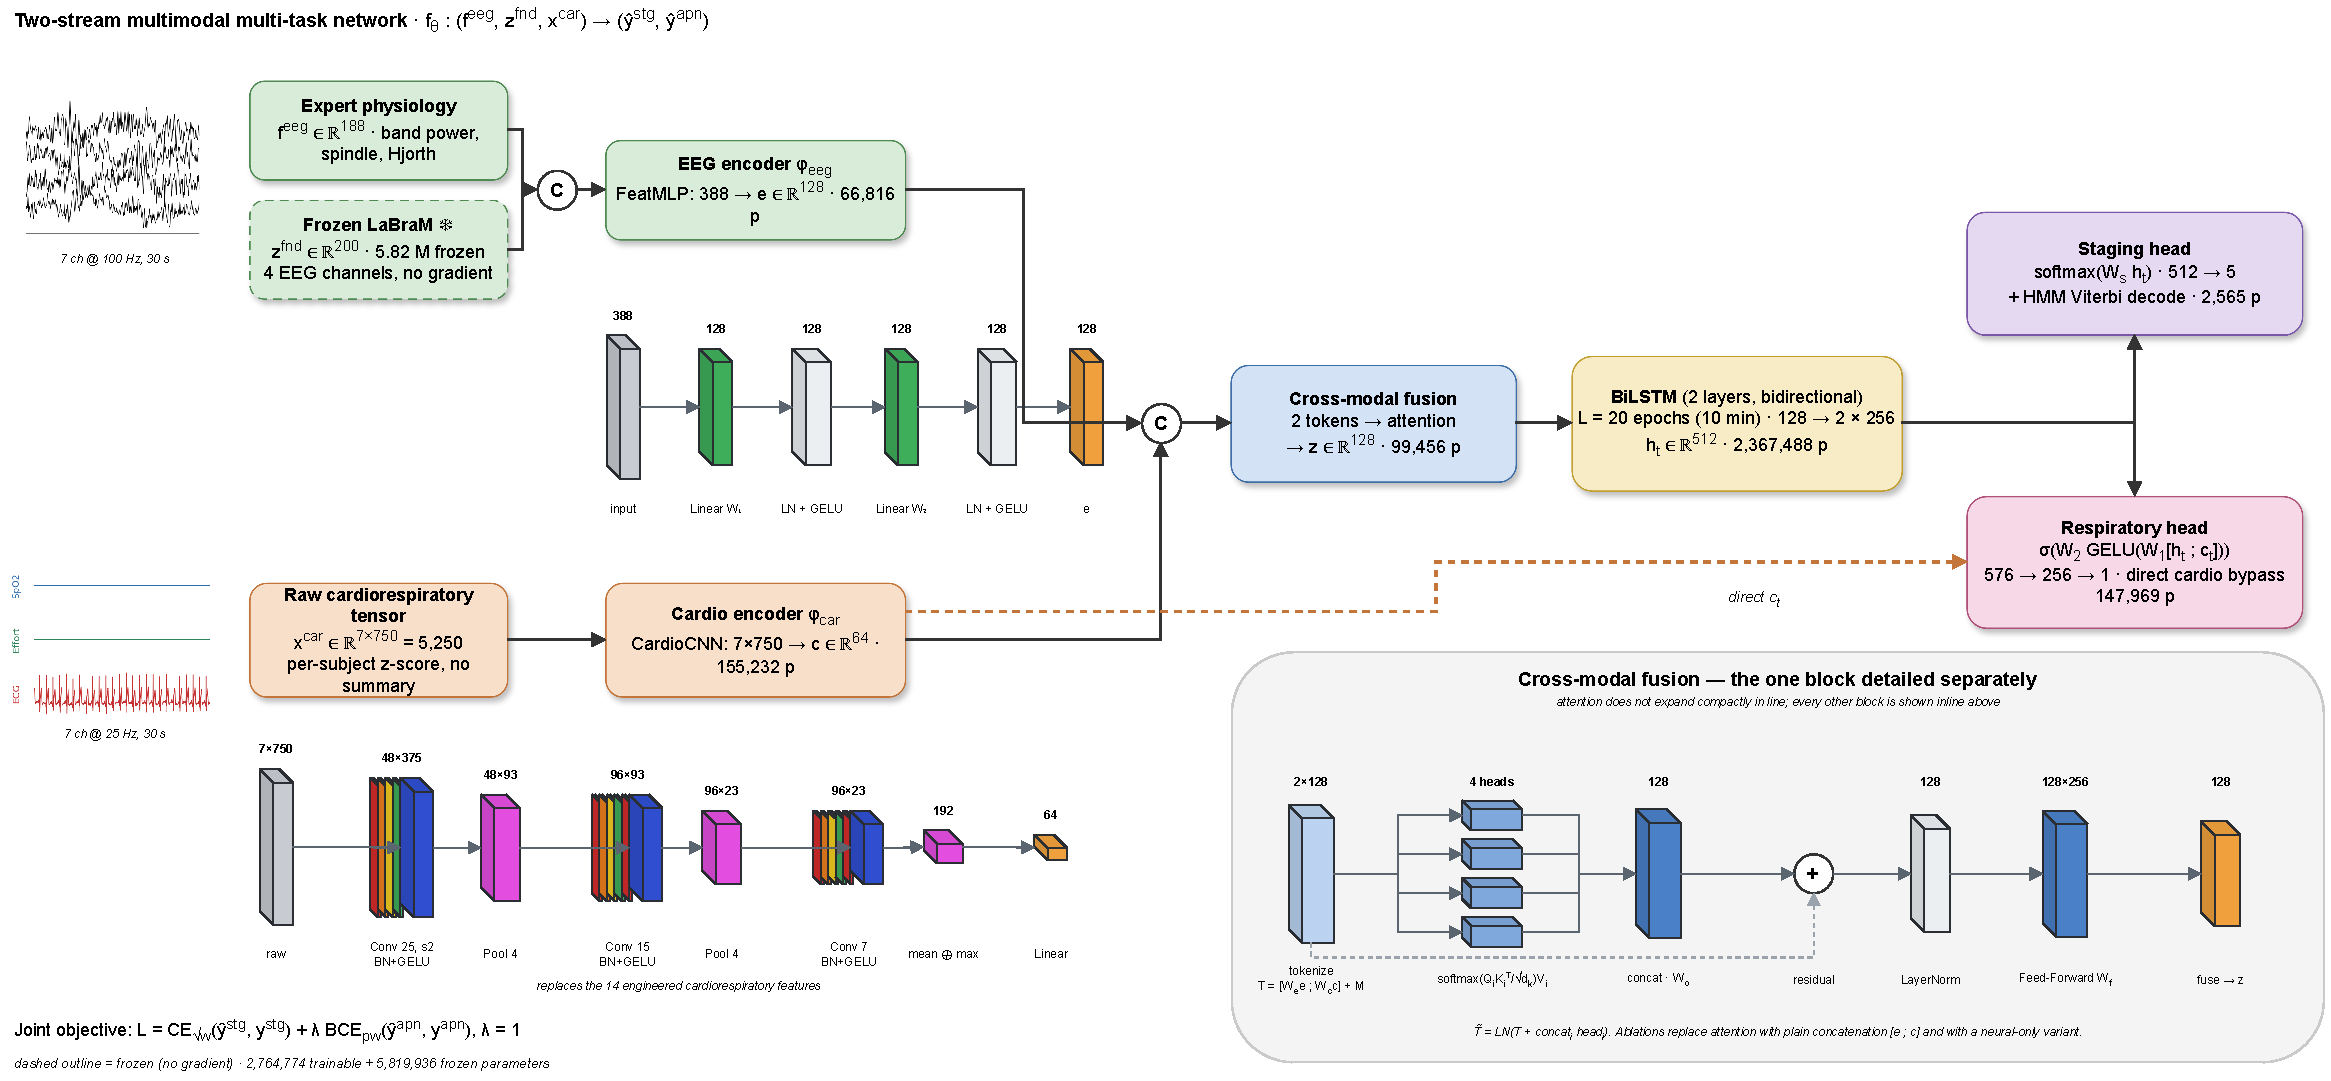
\includegraphics[width=\textwidth]{figures/fig_architecture.pdf}
\caption{The two-stream, multi-task model. (A) The neural features and the cardiorespiratory
features are encoded in parallel, combined by a cross-modal fusion block, and read across the
night by a bidirectional LSTM. A staging head reads the recurrent state; a respiratory head
reads the recurrent state together with a direct copy of the cardiorespiratory embedding, so
oxygen-desaturation and effort cues reach the respiratory decision without passing through the
staging-oriented fusion. (B) Detail of the feature encoder and of the fusion block, which
tokenizes the two modalities, runs four-head attention, and combines the result with a
residual connection.}
\label{fig:arch}
\end{figure*}

\subsection{Physiological feature representations}
\paragraph{Neural features ($188$)}
Per channel we take absolute and relative band powers from the Welch spectrum $P(f)$ in delta
($0.5$--$4$), theta ($4$--$8$), alpha ($8$--$12$), sigma ($12$--$16$), and beta
($16$--$30$)\,Hz; the relative power in band $b$ is
\begin{equation}
\mathrm{RP}_b=\frac{\int_{f\in b}P(f)\,df}{\int_{0.5}^{30}P(f)\,df}.
\end{equation}
We add spectral entropy $H=-\sum_i p_i\log p_i$ with $p_i$ the normalized spectrum, the
$95\%$ spectral-edge frequency, the three Hjorth descriptors~\cite{hjorth1970eeg}, and
time-domain statistics. Sleep spindles are detected on the sigma-band analytic envelope
$e(t)=\lvert\mathcal{H}\{x_\sigma\}(t)\rvert$ from the Hilbert transform $\mathcal{H}$, with
density counted above a per-epoch threshold; slow-wave amplitude, ocular-movement energy on
the EOG, and tonic EMG level complete the set.

\paragraph{Cardiorespiratory features ($14$)}
From the seven cardiorespiratory channels we compute SpO$_2$ mean, minimum, variability, and
desaturation depth (median minus minimum); pulse mean and variability; ECG amplitude and
line-length; airflow amplitude and line-length; thoracic, abdominal, and summed effort
amplitudes; and thoraco-abdominal asynchrony, the loss of coordination between chest and
abdomen that marks an obstructed breath,
\begin{equation}
\mathrm{asyn}_t=\big\lvert\,\mathrm{corr}(x^{\mathrm{tho}}_t,\ x^{\mathrm{abd}}_t)\,\big\rvert .
\end{equation}
Both feature sets are standardized per patient, which removes person-to-person offsets so the
model generalizes across people.

\subsection{Two-stream encoders}
Each stream is a two-layer perceptron with LayerNorm,
\begin{align}
e_t&=\mathrm{GELU}\!\big(\mathrm{LN}(W_2\,\mathrm{GELU}(\mathrm{LN}(W_1\mathbf{f}^{\mathrm{eeg}}_t))) \big)\in\mathbb{R}^{128},\\
c_t&=\mathrm{GELU}\!\big(\mathrm{LN}(U_2\,\mathrm{GELU}(\mathrm{LN}(U_1\mathbf{f}^{\mathrm{car}}_t))) \big)\in\mathbb{R}^{64}.
\end{align}
LayerNorm rather than BatchNorm is used because the recurrent windows are short and mix
patients within a batch, and the cardiorespiratory stream is deliberately narrower because
$14$ slow descriptors carry far less structure than $188$ neural features.

\subsection{Cross-modal fusion}
The two embeddings become two tokens with learned modality-type embeddings
$M\in\mathbb{R}^{2\times D}$, $D=128$,
\begin{equation}
T=\big[\,W_e\,e_t\ ;\ W_c\,c_t\,\big]+M\ \in\ \mathbb{R}^{2\times D}.
\end{equation}
Four-head scaled dot-product attention lets each modality read the other,
\begin{equation}
\begin{aligned}
\mathrm{head}_i&=\mathrm{softmax}\!\Big(\tfrac{(TW^Q_i)(TW^K_i)^{\!\top}}{\sqrt{d_k}}\Big)\,TW^V_i, \\
A&=\big[\mathrm{head}_1;\dots;\mathrm{head}_4\big]W^O,
\end{aligned}
\end{equation}
followed by a residual connection, normalization, and a projection of the two refined tokens,
\begin{equation}
\tilde T=\mathrm{LN}(T+A),\qquad z_t=\mathrm{GELU}\!\big(W_f\,\mathrm{vec}(\tilde T)\big)\in\mathbb{R}^{D}.
\end{equation}
We also evaluate a plain concatenation in place of attention; the two perform alike
(Section~\ref{sec:ablate}), so the reported gain reflects the added modality; the fusion design
contributes little.

\subsection{Temporal decoder and two heads}
Sleep is sequential and respiratory events cluster, so the fused vectors of an $L=20$ epoch
window ($10$ minutes) are read by a two-layer bidirectional LSTM. Each direction runs the
standard recurrence
\begin{align}
i_t&=\sigma(W_i[z_t,h_{t-1}]), & f_t&=\sigma(W_f[z_t,h_{t-1}]),\nonumber\\
o_t&=\sigma(W_o[z_t,h_{t-1}]), & g_t&=\tanh(W_g[z_t,h_{t-1}]),\\
s_t&=f_t\odot s_{t-1}+i_t\odot g_t, & h_t&=o_t\odot\tanh(s_t),\nonumber
\end{align}
and the forward and backward states are concatenated into $h_t\in\mathbb{R}^{256}$. The
staging head is a linear map $\hat y^{\mathrm{stg}}_t=\mathrm{softmax}(W_s h_t)$. The
respiratory head reads $h_t$ together with a direct copy of the per-epoch cardiorespiratory
embedding $c_t$,
\begin{equation}
\hat y^{\mathrm{apn}}_t=\sigma\!\big(W_2\,\mathrm{GELU}(W_1[h_t;c_t])\big).
\end{equation}
This direct connection matters: without it the respiratory decision must survive a fusion
trained mostly for staging, and the fall in oxygen that defines an event is weakened along the
way. The full model holds $0.86$ million parameters.

\subsection{Training and decoding}
The two tasks are trained together with equal weight, $\mathcal{L}=\mathcal{L}^{\mathrm{stg}}+\lambda\,\mathcal{L}^{\mathrm{apn}}$ with $\lambda=1$, combining a class-weighted staging cross-entropy and a positive-weighted respiratory cross-entropy,
\begin{align}
\mathcal{L}^{\mathrm{stg}}&=-\sum_t\sum_{k}w_k\,y^{\mathrm{stg}}_{t,k}\log\hat y^{\mathrm{stg}}_{t,k},\\
\mathcal{L}^{\mathrm{apn}}&=-\sum_t\big[\pi\,a_t\log\hat y^{\mathrm{apn}}_t+(1-a_t)\log(1-\hat y^{\mathrm{apn}}_t)\big].
\end{align}
The staging weights use the square root of inverse class frequency,
$w_k\propto\sqrt{N/(K n_k)}$ for $K=5$ classes with $n_k$ examples, which corrects the scarce
N1 and N3 stages without giving up overall accuracy, and the respiratory term is
positive-weighted by $\pi=n_-/n_+$ to match the $16\%$ event rate. At inference the staging
posteriors are smoothed by a hidden-Markov Viterbi pass whose transition matrix $A^{\mathrm H}$
and prior are counted from the training labels~\cite{chen2024hmm},
\begin{equation}
\delta_t(j)=\max_i\big[\delta_{t-1}(i)+\log A^{\mathrm H}_{ij}\big]+\log\hat y^{\mathrm{stg}}_t(j),
\end{equation}
recovered by back-tracking, which restores the natural persistence of sleep. The respiratory
head is left unsmoothed. Optimization uses AdamW with cosine annealing and early stopping on a
held-out set of patients.

%=====================================================================
\section{Experiments}
\label{sec:results}
\subsection{Protocol and metrics}
All results use ten-fold, patient-independent cross-validation, so no patient appears in both
training and test, and within each training split a disjoint set of patients is held out for
early stopping. Staging is scored by accuracy, macro-F1 $\tfrac{1}{K}\sum_k\mathrm{F1}_k$, and
Cohen's $\kappa$. The respiratory task is scored by the area under the ROC curve (AUC) and
average precision (AP), which suits the $16\%$ event rate.

\subsection{Implementation and hyperparameters}
The model is implemented in PyTorch and trained on a single NVIDIA RTX~2060 GPU (6\,GB) under
Windows, with all randomness seeded to $42$ so that runs are deterministic and reproducible.
Table~\ref{tab:hyper} lists the training configuration, which is identical across all folds, all
baselines we re-implement, and every ablation, so that reported differences come from the model
and not from tuning.

\begin{table}[t]
\caption{Training configuration, shared across all folds, re-implemented baselines, and ablations.}
\label{tab:hyper}
\centering
\small
\begin{tabular}{ll}
\toprule
Setting & Value \\
\midrule
Framework / hardware & PyTorch, NVIDIA RTX~2060 (6\,GB) \\
Optimizer & AdamW \\
Learning rate & $1\times10^{-3}$ \\
Weight decay & $1\times10^{-4}$ \\
LR schedule & cosine annealing \\
Sequence length $L$ & $20$ epochs ($10$\,min) \\
Batch size & $32$ \\
Max epochs / patience & $45$ / $8$ \\
Gradient clipping & $5.0$ \\
Staging class weights & $\sqrt{}$ inverse-frequency \\
Respiratory pos.\ weight & $\pi=n_-/n_+$ \\
Loss balance $\lambda$ & $1.0$ \\
Staging post-processing & HMM Viterbi smoothing \\
Cross-validation & $10$-fold, patient-independent \\
Random seed & $42$ \\
\bottomrule
\end{tabular}
\end{table}

\subsection{Compared Methods}
We compare the model against deep networks evaluated on the same folds: convolutional and
recurrent networks trained from scratch (DeepSleepNet, AttnSleep, a four-channel CNN--BiLSTM), a
network transferred from Sleep-EDF, and a raw-signal convolutional network on all $14$ channels,
alongside the published single-channel baselines for the corpus~\cite{maiti2026isleeps}. We
additionally evaluated a family of classical feature and ensemble pipelines (gradient boosting,
a feature-sequence BiLSTM, a hemispheric graph-attention state-space model, and stacking and
gradient-boosting ensembles); because these only confirm the staging ceiling discussed below,
we report them in the text rather than tabulate them. All numbers are ten-fold
patient-independent, at the hidden-Markov operating point where a model provides one.

\begin{table*}[t]
\caption{Sleep staging on iSLEEPS (ten-fold, patient-independent): the proposed feature-based
model against deep networks trained from scratch, transferred from healthy sleep, or applied to
the raw multichannel signal. ``feat'' marks engineered features; best per column in
\textbf{bold}. Deep architectures built for healthy sleep lose $15$--$20$ points on this stroke
cohort, while the compact feature-based model is the strongest here and the only one that also
detects respiratory events (Table~\ref{tab:ablate}). Classical feature and ensemble pipelines,
which reach a comparable staging ceiling, are summarised in the text.}
\label{tab:bench}
\centering
\begin{tabular*}{\textwidth}{@{\extracolsep{\fill}} l l l c c c c @{}}
\toprule
 & Model & Input & Params\,$\downarrow$ & Acc\,$\uparrow$ & Macro-F1\,$\uparrow$ & $\kappa$\,$\uparrow$ \\
\midrule
\multirow{6}{*}{\emph{Deep networks}}
 & CNN-ResNet18~\cite{maiti2026isleeps}          & 1\,EEG  & $\sim$11\,M  & 0.617 & 0.544 & 0.480 \\
 & DeepSleepNet~\cite{supratak2017deepsleepnet}  & 1\,EEG  & $\sim$21\,M  & 0.615 & 0.567 & 0.483 \\
 & AttnSleep~\cite{eldele2021attnsleep}          & 1\,EEG  & $\sim$0.5\,M & 0.686 & 0.629 & 0.577 \\
 & CNN\,+\,BiLSTM                                & 4\,EEG  & $\sim$0.6\,M & 0.613 & 0.565 & 0.485 \\
 & Sleep-EDF transfer                            & 4\,EEG  & $\sim$0.6\,M & 0.623 & 0.582 & 0.488 \\
 & Raw multimodal CNN                            & 14\,ch  & 0.95\,M     & 0.655 & 0.612 & 0.531 \\
\midrule
\multirow{2}{*}{\shortstack[l]{\emph{Proposed feature-based}\\\emph{multi-task model}}}
 & MM-Net (neural only)              & 7\,ch feat  & 0.77\,M & 0.721 & 0.635 & 0.603 \\
 & \textbf{MM-Net (neural + cardio)} & 14\,ch feat & 0.86\,M & \mmAcc & \textbf{\mmMf} & \textbf{\mmK} \\
\bottomrule
\end{tabular*}
\end{table*}

\subsection{Staging Benchmark and Comparison}
Table~\ref{tab:bench} shows a clear pattern: every deep network, whether trained from scratch,
transferred from healthy sleep, or applied to the raw multichannel signal, stays between $0.61$
and $0.69$ accuracy, $15$ to $20$ points below the same architectures' published accuracy on
healthy sleepers. The compact, feature-based model reaches $\mmAcc$, above every deep baseline,
which matches the concurrent finding that depth alone does not help on this
cohort~\cite{bose2026gap}: with under a hundred patients a convolutional network cannot
rediscover what decades of sleep science already encode in the features. Staging accuracy is
nonetheless capped. The strongest classical pipelines we evaluated reach $0.735$ (a stacking
ensemble) and $0.746$ (a gradient-boosting ensemble), and the published single-channel LSTM
reaches $0.747$; no method exceeds $0.75$, so the task saturates on this cohort regardless of
model family. We therefore do not position the model as a staging leader. What sets it apart is
a second output: it is the only model that also detects respiratory events. A representative held-out night is
shown in Figure~\ref{fig:hypno}: the predicted hypnogram follows the reference through the
night's cycles, and the stage-probability ribbon exposes where the model is confident and where
it hesitates.

\begin{figure*}[t]
\centering
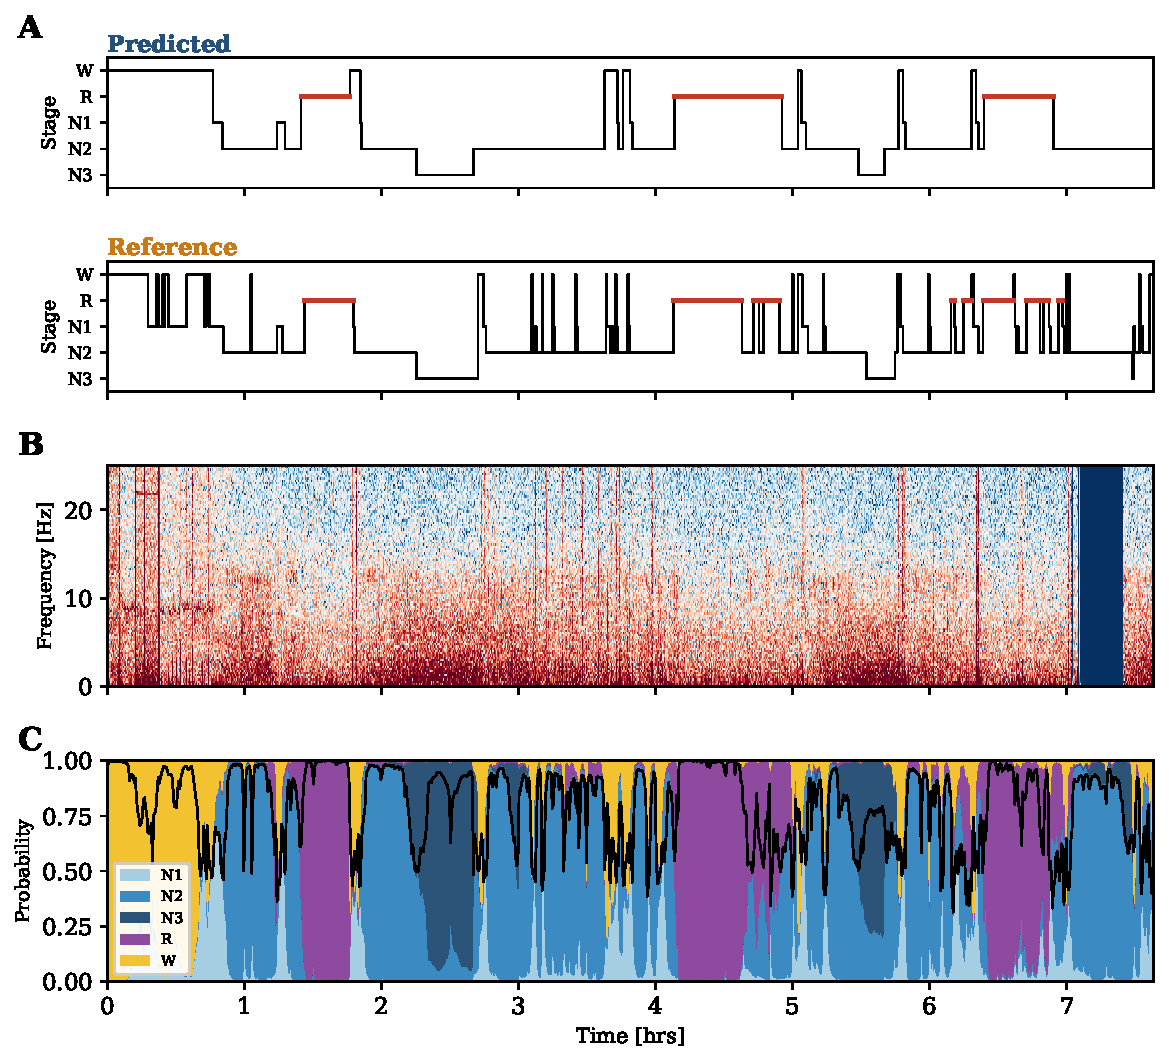
\includegraphics[width=0.86\textwidth]{figures/fig_hypnogram.pdf}
\caption{A representative held-out night (patient SN90, staging accuracy $0.80$).
\textbf{(A)} Predicted and reference hypnograms (REM highlighted). \textbf{(B)} EEG spectrogram
(C4 derivation, $0$--$25$\,Hz). \textbf{(C)} The model's per-epoch stage-probability ribbon; the
black line is the maximum posterior, i.e.\ its confidence. Deep sleep aligns with low-frequency
spectral power, and confidence falls at stage transitions.}
\label{fig:hypno}
\end{figure*}


\subsection{Per-class Staging Performance}
Table~\ref{tab:perclass} breaks staging down by stage. The pattern is the one this cohort
imposes on every method: N2, Wake, and REM are recovered well, N3 is moderate, and N1 is the
hard stage, because it is transient and rare. The raw convolutional network reaches the highest
N1 F1, which fits its sensitivity to short events, while the proposed model leads on the stable
stages. The row-normalised confusion matrix (Fig.~\ref{fig:confusion}) shows
where the errors land: N1 is absorbed mainly into Wake and N2, and part of N3 is read as N2.

\begin{figure}[t]
\centering

\includegraphics[width=0.82\columnwidth]{figures/fig_confusion.pdf}
\caption{Row-normalised confusion matrix for the proposed model (pooled ten-fold test epochs,
hidden-Markov operating point). Errors concentrate on N1, which is absorbed into Wake and N2.}
\label{fig:confusion}
\end{figure}

\begin{table}[t]
\caption{Per-class staging F1 (Wake, N1, N2, N3, REM), ten-fold patient-independent, at the
hidden-Markov operating point, for the proposed model and the raw-signal deep network. Best per
column in \textbf{bold}.}
\label{tab:perclass}
\centering
\setlength{\tabcolsep}{6pt}
\begin{tabular}{lccccc}
\toprule
Model & W\,$\uparrow$ & N1\,$\uparrow$ & N2\,$\uparrow$ & N3\,$\uparrow$ & R\,$\uparrow$ \\
\midrule
Raw multimodal CNN                & 0.74 & \textbf{0.37} & 0.73 & 0.56 & 0.67 \\
MM-Net (neural only)              & 0.77 & 0.24 & 0.78 & 0.68 & 0.70 \\
\textbf{MM-Net (neural + cardio)} & \textbf{0.77} & 0.27 & \textbf{0.78} & \textbf{0.68} & \textbf{0.72} \\
\bottomrule
\end{tabular}
\end{table}

\begin{figure}[t]
\centering
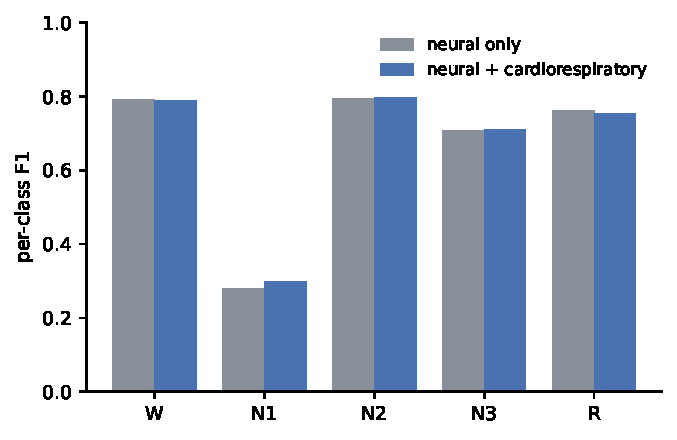
\includegraphics[width=0.86\columnwidth]{figures/fig_mm_perclass.pdf}
\caption{Per-class staging F1 for the neural-only and the neural-plus-cardiorespiratory
model. Adding the cardiorespiratory channels leaves every stage at its full level, including
Wake and REM.}
\label{fig:perclassfig}
\end{figure}

\subsection{Modality-Ablation Grid}
\label{sec:ablate}
This ablation is also our attribution method. Because the model is feature-based and never sees
a raw spectrogram, a gradient heat-map or Grad-CAM would have no faithful spatial support; we
therefore attribute each output by \emph{causal} intervention --- deleting a physiological
channel and measuring the change --- which is a falsifiable test of what each modality
contributes rather than a post-hoc visualization.
The proposed model stages sleep at $\mmAcc$ accuracy ($\kappa$ $\mmK$) and detects respiratory
events at $\mmAuc$ AUC ($\mmAp$ average precision). To test the paper's central claim, that each
modality carries the task its physiology governs, we remove each modality in turn and keep the
rest, on the same folds (Table~\ref{tab:ablate}). The pattern is clean. Removing SpO$_2$ drops
respiratory AUC from $\mmAuc$ to $0.681$ and leaves staging untouched, and removing the whole
cardiorespiratory stream drops it furthest, to $\eegAuc$. Removing the ocular (EOG) channel does
the reverse: staging falls from $\mmAcc$ to $0.712$ while respiratory detection holds. A paired
Wilcoxon test over the ten folds confirms the split: the cardiorespiratory stream changes
respiratory AUC significantly ($0.711$ vs $\eegAuc$, $p=0.004$) but not staging ($p=0.91$). A
cumulative build-up on the respiratory head shows SpO$_2$ alone already reaches the full AUC
($0.711$), so oxygen desaturation carries the read-out and the other channels are largely
redundant for detection. Attention and plain concatenation stage and detect alike, so the gain
comes from the added modality, and the fusion mechanism has little effect.

\begin{figure}[t]
\centering
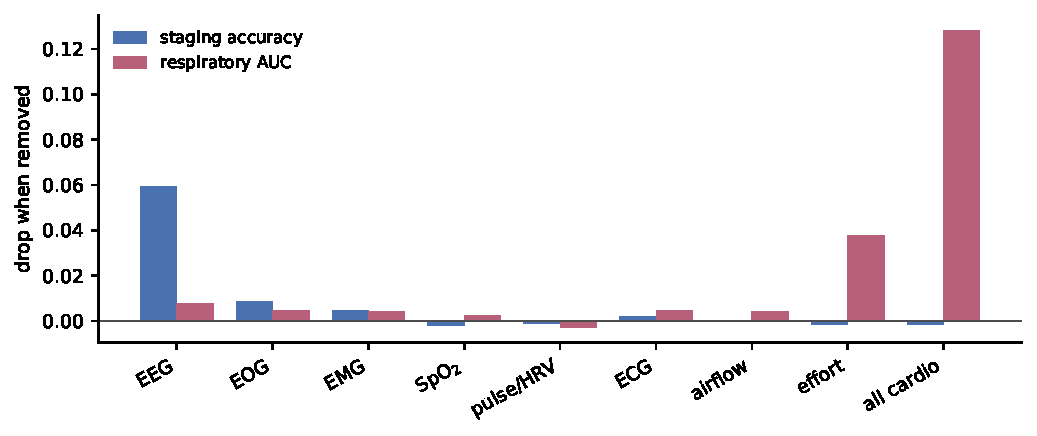
\includegraphics[width=0.98\columnwidth]{figures/fig_ablation.pdf}
\caption{Modality-ablation grid. Staging accuracy (blue) and respiratory AUC (red) as each
modality is removed in turn. Removing SpO$_2$ or the whole cardiorespiratory stream lowers
respiratory AUC and leaves staging flat; removing the ocular channel lowers staging.}
\label{fig:ablationfig}
\end{figure}

\begin{table}[t]
\caption{Modality-ablation grid (leave-one-out), ten-fold patient-independent. Each row removes
one modality and keeps the rest. Cardiorespiratory ablations (SpO$_2$, all cardiorespiratory)
move respiratory AUC and leave staging flat; the ocular (EOG) ablation does the reverse. Largest
effect per column in \textbf{bold}.}
\label{tab:ablate}
\centering
\setlength{\tabcolsep}{8pt}
\begin{tabular}{lcc}
\toprule
Modality removed & Staging acc\,$\uparrow$ & Respiratory AUC\,$\uparrow$ \\
\midrule
none (full model)        & 0.723 & 0.711 \\
SpO$_2$                  & 0.727 & \textbf{0.681} \\
respiratory effort       & 0.728 & 0.726 \\
pulse / HRV              & 0.723 & 0.700 \\
ECG                      & 0.723 & 0.711 \\
airflow                  & 0.722 & 0.704 \\
EOG (ocular)             & \textbf{0.712} & 0.705 \\
EMG (muscle)             & 0.724 & 0.707 \\
all cardiorespiratory    & 0.724 & \textbf{0.673} \\
\bottomrule
\end{tabular}
\end{table}

\subsection{Physiological Validity of the Respiratory Read-out}
\label{sec:noflow}
Because the events were scored from airflow, a model that keyed on the airflow channel would
be right for a trivial reason. Removing the airflow features leaves detection essentially
unchanged, at $\noflowAuc$ AUC (Table~\ref{tab:ablate}), within one fold standard deviation of
the full $\mmAuc$. The model therefore does not lean on the labeling signal. It reads the fall
in blood oxygen, the straining of the chest and abdomen, the beat-to-beat change in the heart,
and the cortical arousal that ends the event. This is the useful regime, because it detects the
bodily consequences of disordered breathing rather than repeating a measurement a technician
has already made.

\subsection{Respiratory Baselines and Per-event-type Detection}
The respiratory task needs real competitors (Table~\ref{tab:resp}), on the same folds and the same $14$
cardiorespiratory features. A clinical desaturation rule reaches $0.596$ AUC, logistic
regression $0.582$, and gradient boosting $0.670$; a random classifier scores $0.160$ average
precision, the event prevalence. The proposed model reaches $\mmAuc$ AUC and $\mmAp$ average
precision, above gradient boosting but by a modest margin, so the contribution is the joint
single pass and the physiological attribution above; we do not claim state-of-the-art
detection accuracy. Detection also separates by event type: the model scores $0.692$ AUC on hypopneas (the
mild, dominant $81\%$ of events), $0.763$ on obstructive apneas, and $0.840$ on central apneas.
It is strongest on the most severe events, and the overall AUC is held down by the abundant
hypopneas.

\begin{table}[t]
\caption{Respiratory-event detection, ten-fold patient-independent. \textit{(a)} Detectors trained
on the $14$ cardiorespiratory features on the same folds; chance-level average precision equals the
event prevalence, $0.160$. \textit{(b)} The proposed model's AUC by event type -- the rarer, more
severe events are detected best. Best per column in \textbf{bold}.}
\label{tab:resp}
\centering
\small
\begin{tabular}{lcc}
\toprule
\multicolumn{3}{l}{\textit{(a) Detection method ($14$ cardiorespiratory features)}}\\
\midrule
Method & AUC\,$\uparrow$ & AP\,$\uparrow$ \\
\midrule
Desaturation rule    & 0.596 & 0.214 \\
Logistic regression  & 0.582 & 0.193 \\
Gradient boosting    & 0.670 & 0.290 \\
MM-Net (proposed)    & \textbf{0.711} & \textbf{0.337} \\
\bottomrule
\end{tabular}

\vspace{4pt}
\begin{tabular}{lcc}
\toprule
\multicolumn{3}{l}{\textit{(b) MM-Net AUC by event type}}\\
\midrule
Event type & Positive epochs & AUC\,$\uparrow$ \\
\midrule
Hypopnea    & 11{,}605 & 0.692 \\
Obstructive & 1{,}661  & 0.763 \\
Central     & 831      & \textbf{0.840} \\
\bottomrule
\end{tabular}
\end{table}

\subsection{Clinical Validation against AHI and Severity}
Aggregating the per-epoch respiratory probability into a per-patient burden and correlating it
with the clinical apnea-hypopnea index (AHI) from the metadata gives a significant positive
association (Spearman $\rho=0.315$, $p=0.002$, $n=96$; Fig.~\ref{fig:ahi}), so the model's output tracks a
clinician's summary measure rather than only an epoch-level score. Staging, in turn, degrades as
sleep-disordered breathing worsens: accuracy falls from $0.770$ in patients with a normal AHI to
$0.708$ in the severe group (Table~\ref{tab:severity}). The pathology that motivates the second output also makes the first
harder, which is the clinical reality of this cohort.

\begin{figure}[t]
\centering
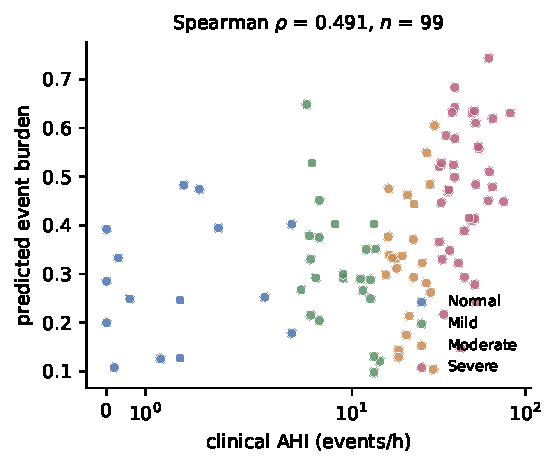
\includegraphics[width=0.86\columnwidth]{figures/fig_ahi.pdf}
\caption{Predicted per-patient event burden (mean respiratory probability) against the clinical
apnea-hypopnea index, coloured by AASM severity band. The positive association (Spearman
$\rho=0.315$, $n=96$) shows the model's output tracks a clinician's summary measure.}
\label{fig:ahi}
\end{figure}

\begin{table}[t]
\caption{Sleep-staging accuracy by sleep-disordered-breathing severity (AASM AHI bands),
ten-fold patient-independent; mean\,$\pm$\,SD across patients ($N=96$). Staging degrades
monotonically as severity rises.}
\label{tab:severity}
\centering
\small
\begin{tabular}{lccc}
\toprule
AHI band & AHI (events/h) & Patients & Staging acc\,$\uparrow$ \\
\midrule
Normal   & $<5$       & 14 & $0.770 \pm 0.064$ \\
Mild     & $5$--$15$  & 22 & $0.730 \pm 0.077$ \\
Moderate & $15$--$30$ & 23 & $0.712 \pm 0.103$ \\
Severe   & $\geq 30$  & 37 & $0.708 \pm 0.091$ \\
\bottomrule
\end{tabular}
\end{table}

\subsection{Model Complexity and Capability}
Table~\ref{tab:cost} sets the proposed model beside representative alternatives on size and
capability. A single compact network, under a million parameters and an order of magnitude
smaller than the raw-signal transformers, delivers both a competitive stage and a respiratory
read-out from one pass over the recording. None of the staging-only models, at any size, can
supply the second output.

\begin{table}[t]
\caption{Model size and clinical capability. The proposed model is compact and is the only one
that produces both a stage and a respiratory-event label.}
\label{tab:cost}
\centering
\setlength{\tabcolsep}{4pt}
\begin{tabular}{lccc}
\toprule
Model & Input & Params\,$\downarrow$ & Outputs \\
\midrule
CNN-ResNet18~\cite{maiti2026isleeps}      & 1\,EEG      & $\sim$11\,M & stage \\
DeepSleepNet~\cite{supratak2017deepsleepnet} & 1\,EEG   & $\sim$21\,M & stage \\
Feature-sequence BiLSTM                   & 7\,ch feat  & 1.2\,M      & stage \\
Raw multimodal CNN                        & 14\,ch      & 0.95\,M     & stage + apnea \\
\textbf{MM-Net (proposed)}                & 14\,ch feat & \textbf{0.86\,M} & \textbf{stage + apnea} \\
\bottomrule
\end{tabular}
\end{table}

%=====================================================================
\section{Discussion}
The result is a single model that reads the whole sleeping body and speaks to two clinical
questions at once, in the population where both matter. The learned per-epoch embedding
(Fig.~\ref{fig:tsne}) separates cleanly by sleep stage while the respiratory structure stays
diffuse, mirroring the strong staging and the modest respiratory AUC.

\begin{figure*}[t]
\centering
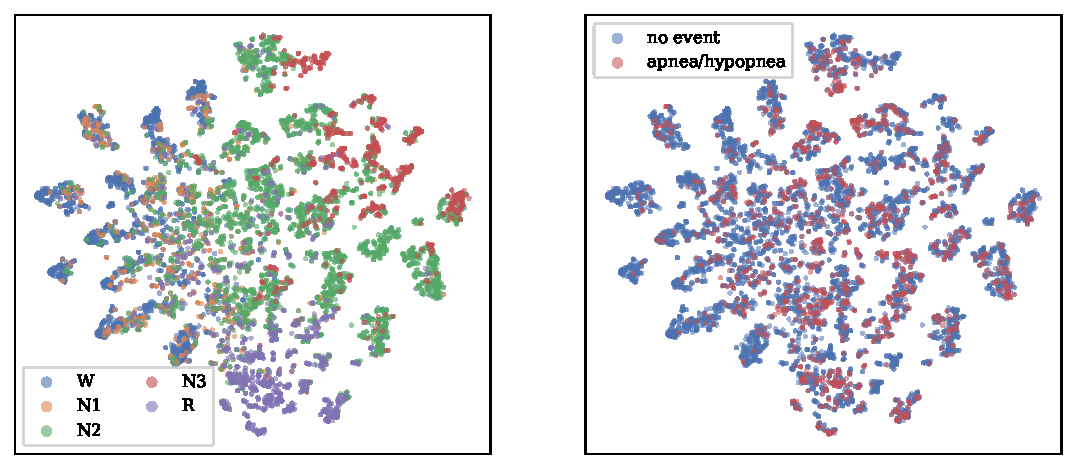
\includegraphics[width=0.92\textwidth]{figures/fig_tsne.pdf}
\caption{Two-dimensional t-SNE of the model's per-epoch embeddings (pooled test epochs).
\textbf{Left:} coloured by sleep stage -- Wake, N2, N3, and REM form distinct territories while
N1 is diffuse. \textbf{Right:} coloured by respiratory-event label -- events are spread across
the manifold, consistent with the modest detection AUC.}
\label{fig:tsne}
\end{figure*} Staging accuracy on this cohort saturates
below $0.75$ for every model family we evaluated, and the proposed model reaches $\mmAcc$ while
adding a respiratory capability the staging models lack. The respiratory
read-out does not depend on the labeling channel: it survives deletion of the airflow channel and
rests on oxygen desaturation, effort, and arousal, the same signs a physician reads at the
bedside.

The $0.72$ staging figure should be judged on this cohort, where healthy-sleep accuracy does not transfer. Deep
architectures developed on healthy sleepers collapse here: DeepSleepNet reaches $0.615$,
CNN-ResNet18 $0.617$, and a network pretrained on the healthy Sleep-EDF corpus and applied to
this cohort $0.623$, each roughly fifteen to twenty points below its healthy accuracy of about
$0.85$. The injured brain distorts the very micro-events, spindles, slow waves, and atonia, that
those models learned to read. What holds up is physiologically grounded modeling on engineered
features, at $0.72$ to $0.75$, which matches the published baseline on this corpus. The lesson is
that healthy-sleep deep learning fails on the injured brain, and this cohort requires
cohort-specific, physiologically grounded, multimodal modeling.

The study also draws a clean physiological line. The cortical channels carry sleep staging, and
the cardiorespiratory channels carry breathing, and the model places each where it belongs
rather than blurring them. That the neural and multimodal variants stage alike is the expected
outcome: the second modality adds a new capability while leaving staging unchanged. We view this separation as a strength for
clinical use, because a reader can trust that the respiratory output reflects breathing and the
staging output reflects the brain.

\subsection{Limitations}
The evidence comes from a single center and the $96$ patients with
complete cardiorespiratory channels; external, multi-center validation is required before
clinical use. Respiratory detection, at $\mmAuc$ AUC, is a useful signal but not yet a
screening-grade one, and it is scored at the epoch level rather than per event. Staging sits at
the cohort ceiling, so the model does not raise staging accuracy over strong classical
pipelines. Finally, the model is feature-based: it inherits the assumptions of the engineered
representations and is not an end-to-end raw-signal learner, a deliberate trade for data
efficiency on a small cohort.

\subsection{Future Work}
Two directions follow naturally. Event-level metrics, such as sensitivity per event and false
alarms per hour, would sit beside the epoch-level AUC and speak more directly to a sleep
technician, and finer modeling of the breathing waveforms is likely to raise the respiratory
number further. Linking the multimodal representation to stroke severity and recovery is the
larger opportunity, and one the cardiorespiratory signal is well placed to serve.

%=====================================================================
\begin{table*}[t]
\caption{Recent single-channel sleep-staging methods: the accuracy each reports on healthy or
general cohorts, set against its accuracy on the subacute-stroke cohort (iSLEEPS) for the two
architectures we re-implemented. Healthy-cohort staging reaches $0.82$--$0.88$; the same
architectures fall to $0.62$--$0.69$ on stroke, while the proposed multimodal model reaches
$\mmAcc$ on stroke and additionally detects respiratory events at $\mmAuc$ AUC (no staging
method produces a respiratory output). A dash marks a value we did not evaluate.}
\label{tab:litreview}
\centering
\small
\begin{tabular*}{\textwidth}{@{\extracolsep{\fill}} l c p{7.2cm} c c @{}}
\toprule
Method & Year & Approach & Reported acc (dataset) & On iSLEEPS \\
\midrule
DeepSleepNet~\cite{supratak2017deepsleepnet} & 2017 & Two representation-learning CNNs followed by a bidirectional LSTM sequence model, single-channel EEG. & $0.82$ (Sleep-EDF) & $0.615$ \\
AttnSleep~\cite{eldele2021attnsleep} & 2021 & Multi-resolution CNN with multi-head self-attention over epochs, single-channel EEG. & $0.844$ (Sleep-EDF) & $0.686$ \\
SleepTransformer & 2022 & Transformer encoder with epoch-level interpretability and uncertainty estimates. & $0.877$ (SHHS) & -- \\
1D-ResNet-SE-LSTM & 2023 & Residual network with squeeze-and-excitation blocks and an LSTM on raw EEG. & $0.864$ (Sleep-EDF) & -- \\
Micro SleepNet & 2023 & Lightweight convolutional model for real-time mobile staging. & $0.833$ (SHHS) & -- \\
AT-BiLSTM & 2024 & Attention-augmented bidirectional LSTM, single-channel EEG. & $0.838$ (Sleep-EDF) & -- \\
\midrule
\textbf{MM-Net (proposed)} & -- & Two feature streams (neural and cardiorespiratory) fused into a BiLSTM that jointly stages sleep and detects respiratory events from the full polysomnogram. & -- & $\mathbf{0.722}$ \\
\bottomrule
\end{tabular*}
\end{table*}

\section{Conclusion}
We built a model that reads the full polysomnogram of stroke patients and, from one pass,
stages their sleep and detects their respiratory events. Deep networks built for healthy sleep
collapse to $0.61$--$0.69$ accuracy on this cohort, so its $\mmAcc$ staging accuracy is at the
cohort ceiling for every model family. The contribution is the second output, a respiratory
read-out at $\mmAuc$ AUC that survives removal of the airflow channel, showing it reads the
underlying physiology. Reading the whole recording gives the model a second clinical voice in the
population that needs it most. Code and features are released.

%=====================================================================
\section*{Data and Code Availability}
The iSLEEPS corpus is publicly available (Zenodo, DOI 10.5281/zenodo.14873844; and the
india-data.org portal) as described by Maiti \textit{et al.}~\cite{maiti2026isleeps}. Our
code, engineered features, and reproduction notebook are released at
\url{https://github.com/wshuv-o/isleeps-sleep-staging}.

\section*{Ethics}
The iSLEEPS data collection was approved by the NIMHANS Institutional Ethics Committee
(No.\ NIMHANS/34th IEC (BS\&NS DIV.)/2022, dated 05.02.2022)~\cite{maiti2026isleeps}. This work
is a secondary analysis of the de-identified public release and required no additional
enrollment.

\section*{Funding}
The authors received no specific funding for this work.

%=====================================================================
\section*{Acknowledgment}
The authors thank the iSLEEPS investigators for releasing the corpus.

\bibliographystyle{IEEEtran}
\bibliography{references}

\end{document}
